\documentclass[a4paper]{article}
\usepackage[english]{babel}
\usepackage[utf8]{inputenc}
\usepackage{textcomp}
\usepackage{amsmath}
\usepackage{gensymb}
\usepackage{physics}
\usepackage{graphicx}
\usepackage[colorinlistoftodos]{todonotes}
\usepackage{xcolor}
\usepackage{array}
\usepackage{tabularx}
\usepackage{tikz}
\usepackage{pgfplots}
\usepackage{framed}
\usepackage{xfrac}
\usepackage[most]{tcolorbox}
\usepackage{fix-cm}
\usepackage{cancel}
\usepackage[margin=0.5in]{geometry}
\usetikzlibrary{quotes,angles}
\usetikzlibrary{decorations.pathreplacing}
\usetikzlibrary{calc}
\usepgfplotslibrary{fillbetween}

\let\phi\varphi
\let\bf\textbf
\colorlet{shadecolor}{orange!15}
\pgfplotsset{compat=1.18}
\newcommand\der[2]{\frac{d #1}{d #2}}
\newcommand\Deltat{\Delta t}
\newcommand\rads{\text{ rad\;s}^{-1}}
\newcommand\radss{\text{ rad\;s}^{-2}}
\newcommand\rad{\text{ rad}}
\newcommand\s{\text{ s}}
\newcommand\m{\text{ m}}
\newcommand\J{\text{ J}}
\newcommand\ms{\text{ ms}^{-1}}
\newcommand\mss{\text{ ms}^{-2}}
\newcommand\kg{\text{ kg}}
\newcommand\kgms{\text{ kg\;ms}^{-1}}
\newcommand\kgmm{\text{ kg\;m}^{-2}}
\newcommand{\AxisRotator}[1][rotate=0]{%
    \tikz [x=0.25cm,y=0.60cm,line width=.2ex,-stealth,#1] \draw (0,0) arc (-150:150:1 and 1);%
}
\def\centerarc[#1](#2)(#3:#4:#5){\draw[#1] ($(#2)+({#5*cos(#3)},{#5*sin(#3)})$) arc (#3:#4:#5)}
% Syntax: \centerarc[draw options] (center) (initial angle:final angle:radius);

\title{Fixed-Axis Rotation}
\author{OpenStax University Physics Vol. 1}
\date{}

\begin{document}
\setcounter{section}{10}
\maketitle
\subsection{Rotational Variables}
\noindent\bf{Angular Velocity}
\vspace{2mm}\\
Uniform circular motion is motion in a circle at constant speed, although this is the simplest case of rotational motion, it is used here to introduce rotational variables.\par
The figure shows a particle moving in a circle. Its position vector from the origin of the circle to the particle sweeps out the angle $\theta$, which increases in the counterclockwise direction as the particle moves along its path. The angle $\theta$ is called the angular position of the particle. As the particle moves, it traces an arc length $s$.
\begin{center}
    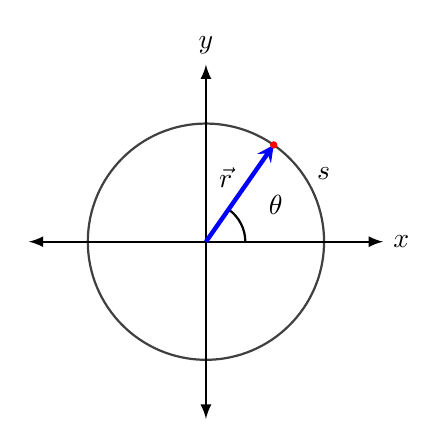
\begin{tikzpicture}[scale=1.5]
        %%% COORDINATES %%%
        \draw (0,0) coordinate (o);
        \draw ({cos(55)},{sin(55)}) coordinate (a);
        \draw ({cos(55)},0) coordinate (b);

        %%% AXES & CIRCLE %%%
        \draw[thick,draw=black!75] (0,0) circle (1);
        \draw[<->,thick,-latex] (0,0)--(1.5,0) node[right]{$x$};
        \draw[<->,thick,-latex] (0,0)--(0,1.5) node[above]{$y$};
        \draw[<->,thick,-latex] (0,0)--(-1.5,0);
        \draw[<->,thick,-latex] (0,0)--(0,-1.5);

        %%% POSITION VECTOR & ANGLE %%%
        \draw pic["$\theta$",draw=black,thick,-,angle eccentricity=2,angle radius=0.5cm]{angle=b--o--a};
        \draw[->,ultra thick,draw=blue,-stealth] (0,0)--node[left,xshift=0.5mm,yshift=2mm]{$\vec{r}$}({cos(55)},{sin(55)});

        \centerarc[red,very thick](0,0)(0:55:1);
        \node at ({1.15*cos(30)},{1.15*sin(30)}){$s$};
        \filldraw[red] ({cos(55)},{sin(55)}) circle (0.75pt);
    \end{tikzpicture}
\end{center}
The angle is related to the radius of the circle and the arc length by 
\begin{equation}
    \theta = \frac{s}{r}
\end{equation}
The angle $\theta$, the angular position of the particle moving along its path has units of radians (rad). As the particle moves along its circular path, its angular position changes and it undergoes angular displacements $\Delta\theta$.\par\vspace{1mm}
\noindent We can assign vectors to the quantities in equation 1, the angle $\vec{\theta}$ is a vector out of the page. The angular position vector $\vec{r}$ and the arc length vector $\vec{s}$ both lie in the plane of the page, they are related by:
\begin{equation}
    \vec{s} = \vec{\theta} \times \vec{r}
\end{equation}
The arc length is the cross product of the angle vector and the position vector
\begin{center}
    \begin{tikzpicture}[scale=2]
        \draw[->,-latex] (0,0)--(1,0) node[right]{$y$};
        \draw[->,-latex] (0,0)--(0,1) node[above]{$z$};
        \draw[->,-latex] (0,0)--(-{cos(45)},-{sin(45)}) node[left]{$x$};

        \draw[->,very thick,-stealth] (0,0)--node[right]{$\vec{\theta}$}(0,0.75);
        \draw[->,very thick,-stealth] (0,0)--node[below,xshift=-2mm,yshift=0.5mm]{$\vec{r}$}({0.7*cos(65)},{-0.7*cos(65)});
        \draw[->,very thick,-stealth,draw=red] ({0.7*cos(65)},{-0.7*cos(65)})--node[right,yshift=-1mm,xshift=-0.5mm]{$\vec{s}$}({0.7*cos(65) + 0.28},{-0.7*cos(65) + 0.28});
    \end{tikzpicture}
\end{center}
The magnitude of the angular velocity, denoted by $\omega$, is the time rate of change of the angle $\theta$ as the particle moves in a circular path. The instantaneous angular velocity, defined as the limit as $\Delta t \to 0$ of the average angular velocity $\bar{\omega} = \frac{\Delta\theta}{\Delta t}$
\begin{equation}
    \omega = \lim\limits_{\Delta t \to 0}\frac{\Delta\theta}{\Delta t} = \frac{d\theta}{dt}
\end{equation}
Where $\theta$ is the angle of rotation. The units of angular velocity are radians per second (rad\;s$^{-1}$). Angular velocity can also be referred to as the rotation rate in radians per second. In many cases, rotation rate is given in revolutions/s or cycles/s, to find angular velocity, multiply revolutions/s by $2\pi$ (since there are $2\pi$ radians per revolution). Since a positive angle in a circle is counterclockwise, we take counterclockwise rotations as being positive and clockwise rotations as negative.\vspace{1mm}\par
\noindent We can see how angular velocity is related to the tangential speed of the particle by differentiating equation 1 with respect to time. Equation 1 can be rewritten as:
\begin{align*}
    s = \theta r
\end{align*}
\newpage
\noindent Taking the derivative with respect to time and noting that the radius $r$ is constant gives:
\begin{align*}
    \der{s}{t} = \der{}{t}(r\theta) = \theta\der{r}{t} + r\der{\theta}{t} = r\der{\theta}{t}
\end{align*}
Where $\theta\der{r}{t} = 0$. Here, $\der{s}{t}$ is just the tangential speed $v_t$ of the particle moving in a circular path. Using equation 3 we arrive at:
\begin{equation}
    v_t = r\omega
\end{equation}
The tangential speed of the particle is its angular velocity times the radius of the circle. The tangential speed of the particle increases with its distance from the axis of rotation for a constant angular velocity. The figure shows two particles placed at different radii on a rotating disk with constant angular velocity. As it rotates, the tangential speed increases linearly with the radius from the axis of rotation. We see that $v_1 = r_1\omega_1$ and $v_2 = r_2\omega_2$. The disk has a constant angular velocity so $\omega_1 = \omega_2$. This means that $\frac{v_1}{r_1} = \frac{v_2}{r_2}$ or $v_2 = \big(\frac{r_2}{r_1}\big)$. Thus, since $r_2 > r_1$, $v_2 > v_1$
\begin{center}
    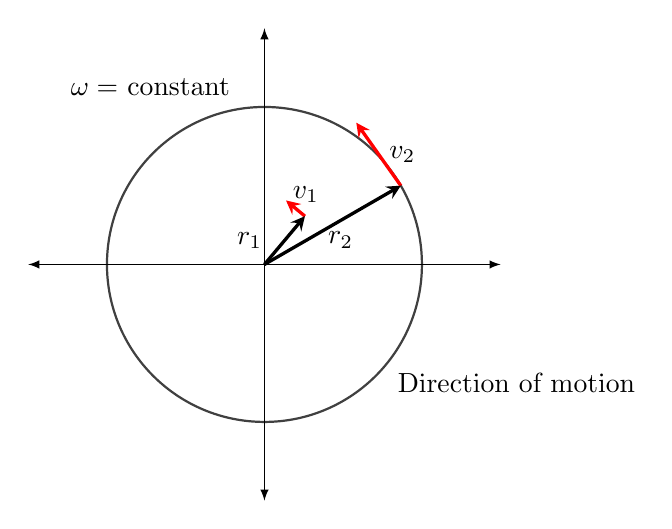
\begin{tikzpicture}[scale=2]
        %%% COORDINATES %%%
        \draw (0,0) coordinate (O);
        \draw ({cos(30)},{sin(30)}) coordinate (a);
        \draw ({0.4*cos(50)},{0.4*sin(50)}) coordinate (b);

        %%% AXES & CIRCLE %%%
        \draw[thick,draw=black!75] (0,0) circle (1);
        \draw[->,-latex] (O)--(1.5,0);
        \draw[->,-latex] (O)--(-1.5,0);
        \draw[->,-latex] (O)--(0,1.5);
        \draw[->,-latex] (O)--(0,-1.5);

        %%% LINES %%%
        \draw[->,very thick,-stealth,draw=red] (a)--node[right]{$v_2$}({cos(30) - 0.4*cos(45)},{sin(30) + 0.4});
        \draw[->,very thick,-stealth,draw=red] (b)--({0.4*cos(50) - 0.17*cos(45)},{0.4*sin(50) + 0.1}) node[right,yshift=0.75mm,xshift=-0.5mm]{$v_1$};
        \draw[->,very thick,-stealth] (O)--node[below,xshift=1mm,yshift=0.5mm]{$r_2$}(a);
        \draw[->,very thick,-stealth] (O)--node[left,xshift=-1.5mm]{$r_1$}(b);

        \node at ({-1.45*cos(60)},{1.3*sin(60)}){$\omega =$ constant};

        \centerarc[->,black!50,thick,-stealth](0,0)(-30:-10:1.1);
        \centerarc[->,black!50,thick,-stealth](0,0)(60:80:1.1);
        \centerarc[->,black!50,thick,-stealth](0,0)(150:170:1.1);
        \centerarc[->,black!50,thick,-stealth](0,0)(240:260:1.1);
        \node at (1.6,-0.75){Direction of motion};
    \end{tikzpicture}
\end{center}
Similar to equation 2, one can state a cross product relation to the vector of the tangential velocity as stated in equation 4, therefore:
\begin{equation}
    \vec{v} = \vec{\omega} \times \vec{r}
\end{equation}
The tangential velocity is the cross product of the angular velocity and the position vector as shown below. On the left we see that with the angular velocity in the $+z$ direction, the rotation in the $xy$ plane is counterclockwise. On the right, the angular velocity is in the $-z$ direction, which gives a clockwise rotation in the $xy$ plane.
\begin{center}
    \begin{tikzpicture}[scale=2]
        \draw[->,-latex] (0,0)--(1,0) node[right]{$y$};
        \draw[->,-latex] (0,0)--(0,1) node[above]{$z$};
        \draw[->,-latex] (0,0)--(-{cos(45)},-{sin(45)}) node[left]{$x$};

        \draw[->,very thick,-stealth] (0,0)--node[right]{$\vec{\omega}$}(0,0.75);
        \draw[->,very thick,-stealth,draw=red] ({0.7*cos(65)},{-0.7*cos(65)})--node[right,yshift=-1mm,xshift=-0.5mm]{$\vec{v}$}({0.7*cos(65) + 0.26},{-0.7*cos(65) + 0.26});
        \draw[->,very thick,-stealth] (0,0)--node[below,xshift=-2mm,yshift=0.5mm]{$\vec{r}$}({0.7*cos(65)},{-0.7*cos(65)});
    \end{tikzpicture}
    \hspace{15mm}
    \begin{tikzpicture}[scale=2]
        \draw[->,-latex] (0,0)--(1,0) node[right]{$y$};
        \draw[->,-latex] (0,0)--(0,1) node[above]{$z$};
        \draw[->,-latex] (0,0)--(-{cos(45)},-{sin(45)}) node[left]{$x$};

        \draw[->,very thick,-stealth] (0,0)--node[left]{$\vec{\omega}$}(0,-0.75);
        \draw[->,very thick,-stealth,draw=red] ({0.7*cos(65)},{-0.7*cos(65)})--node[right,yshift=-1mm,xshift=-0.5mm]{$\vec{v}$}({0.7*cos(65) - 0.26},{-0.7*cos(65) - 0.26});
        \draw[->,very thick,-stealth] (0,0)--node[above,yshift=-1.5mm,xshift=1.5mm]{$\vec{r}$}({0.7*cos(65)},{-0.7*cos(65)});
    \end{tikzpicture}
\end{center}
\begin{shaded}
    \underline{\bf{Example 10.1:} Rotation of a Flywheel}
    \vspace{2mm}\\
    A flywheel rotates such that it sweeps out an angle at the rate of $\theta = \omega t = (45.0\text{ rad\;s}^{-1})t$ radians. The wheel rotates counterclockwise when viewed in the plane of the page.
    \begin{enumerate}
        \item[(a)] What is the angular velocity $\omega$ of the flywheel?
        \vspace{1mm}\\
        $\displaystyle \omega = \der{\theta}{t} = 45$ rad\;s$^{-1}$, angular velocity is constant
        \item[(b)] What direction is the angular velocity?
        \vspace{1mm}\\
        The direction of rotation is counterclockwise, so the direction of angular velocity is $+z$
        \item[(c)] How many radians does the flywheel rotate through in 30 s?
        \vspace{1mm}\\
        $\displaystyle \theta(t) = \omega t \to \Delta\theta = \theta(30$ s$) - \theta(0$ s$) = \theta(30$ s$) \to (45.0$ rad\;s$^{-1})(30$ s$) = 1350.0$ rad
        \item[(d)] What is the tangential speed of a point on the flywheel 10 cm from the axis of rotation
        \vspace{1mm}\\
        $v_t = r\omega = (0.1$ m$)(45.0$ rad\;s$^{-1}) = 4.5$ ms$^{-1}$
    \end{enumerate}
\end{shaded}
\newpage
\noindent\bf{Angular Acceleration}
\vspace{2mm}\\
For describing situations where $\omega$ changes, we need to define angular acceleration. The faster the change in $\omega$, the greater the angular acceleration. Instantaneous angular acceleration $\alpha$ is defined as the derivative of angular velocity with respect to time:
\begin{equation}
    \alpha = \lim_{\Delta t \to 0}\frac{\Delta\omega}{\Delta t} = \der{\omega}{t} = \frac{d^2\theta}{dt^2}
\end{equation}
Where we have taken the limit of the average angular acceleration $\bar{\alpha} = \frac{\Delta\omega}{\Delta t}$ as $\Delta t \to 0$. The units of angular acceleration are radians/s per second, or rad\;s$^{-2}$. 
\vspace{1mm}\par
\noindent In the same way that the vector associated with angular velocity $\vec{\omega}$ was defined, we can define $\vec{\alpha}$, the vector associated with angular acceleration. If the angular velocity is along the $+z$ axis and $\der{\omega}{t}$ is positive, the angular acceleration $\vec{\alpha}$ is positive and points along the $+z$ axis, if $\der{\omega}{t}$ is negative, the angular acceleration is negative and points along the $-z$ axis.

\begin{center}
    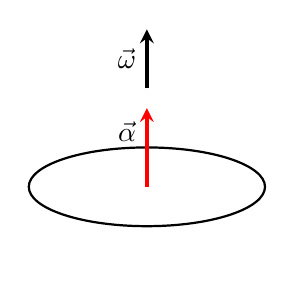
\begin{tikzpicture}
        \draw[thick] (0,0) ellipse (1.5 and 0.5);
        \draw (0,0) coordinate (O);
        \draw[->,very thick,-stealth,draw=red] (O)--node[left,yshift=2mm]{$\vec{\alpha}$}(0,1);
        \draw[->,very thick,-stealth] (0,1.25)--node[left]{$\vec{\omega}$}(0,2);
        \centerarc[->,black!50,thick,-stealth](0,0)(-10:10:1.7);
        \node at (0,-1){};
    \end{tikzpicture}
    \hspace{15mm}
    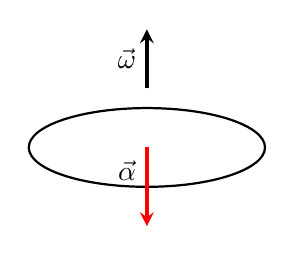
\begin{tikzpicture}
        \draw[thick] (0,0) ellipse (1.5 and 0.5);
        \draw (0,0) coordinate (O);
        \draw[->,very thick,-stealth,draw=red] (O)--node[left,yshift=2mm]{$\vec{\alpha}$}(0,-1);
        \draw[->,very thick,-stealth] (0,0.75)--node[left]{$\vec{\omega}$}(0,1.5);
        \centerarc[->,black!50,thick,-stealth](0,0)(-10:10:1.7);
    \end{tikzpicture}
\end{center}
The tangential acceleration vector can be expressed as a cross product of the angular acceleration and position vectors. This equation can be found by taking the derivative of equation 5
\begin{equation}
    \vec{a} = \vec{\alpha} \times \vec{r}
\end{equation}
The vector relationships for angular acceleration and tangential acceleration are shown below
\begin{center}
    \begin{tikzpicture}[scale=2]
        \draw[->,-latex] (0,0)--(1,0) node[right]{$y$};
        \draw[->,-latex] (0,0)--(0,1) node[above]{$z$};
        \draw[->,-latex] (0,0)--(-{cos(45)},-{sin(45)}) node[left]{$x$};

        \draw[->,very thick,-stealth] (0,0)--node[right]{$\vec{\alpha}$}(0,0.75);
        \draw[->,very thick,-stealth,draw=red] ({0.7*cos(65)},{-0.7*cos(65)})--node[right,yshift=-1mm,xshift=-0.5mm]{$\vec{a}$}({0.7*cos(65) + 0.26},{-0.7*cos(65) + 0.26});
        \draw[->,very thick,-stealth] (0,0)--node[below,xshift=-2mm,yshift=0.5mm]{$\vec{r}$}({0.7*cos(65)},{-0.7*cos(65)});
    \end{tikzpicture}
    \hspace{15mm}
    \begin{tikzpicture}[scale=2]
        \draw[->,-latex] (0,0)--(1,0) node[right]{$y$};
        \draw[->,-latex] (0,0)--(0,1) node[above]{$z$};
        \draw[->,-latex] (0,0)--(-{cos(45)},-{sin(45)}) node[left]{$x$};

        \draw[->,very thick,-stealth] (0,0)--node[left]{$\vec{\alpha}$}(0,-0.75);
        \draw[->,very thick,-stealth,draw=red] ({0.7*cos(65)},{-0.7*cos(65)})--node[right,yshift=-1mm,xshift=-0.5mm]{$\vec{a}$}({0.7*cos(65) - 0.26},{-0.7*cos(65) - 0.26});
        \draw[->,very thick,-stealth] (0,0)--node[above,yshift=-1.5mm,xshift=1.5mm]{$\vec{r}$}({0.7*cos(65)},{-0.7*cos(65)});
    \end{tikzpicture}
\end{center}
Tangential acceleration of a point on a rotating body at a distance from the axis of rotation can be related in the same way as tangential velocity and angular velocity. Differentiating equation 4 with respect to time (the radius $r$ is constant) gives:
\begin{equation}
    a_t = r\alpha
\end{equation}
The tangential acceleration $a_t$ is the radius times the angular acceleration
\begin{shaded}
    \underline{\bf{Example 10.2:} A Spinning Bike Wheel}
    \vspace{2mm}\\
    A bicycle mechanic mounts a bicycle on the repair stand and starts the rear wheel spinning from rest to a final angular velocity of 250 rpm in 5.00 s.
    \begin{enumerate}
        \item[(a)] Calculate the average angular acceleration in rad\;s$^{-2}$
        \begin{align*}
            \displaystyle \bar{\alpha} = \frac{\Delta\omega}{\Delta t} = \frac{250\text{ rpm}}{5.00\text{ s}}
        \end{align*}
        Converting from rpm to rad\;s$^{-1}$:
        \begin{align*}
            \Delta\omega = 250\frac{\text{rev}}{\text{min}} \cdot \frac{2\pi\text{ rad}}{\text{rev}} \cdot \frac{1\text{ min}}{60\text{ s}} = 26.2\text{rad\;s}^{-1}
        \end{align*}
        Entering this back into the expression for $\alpha$ gives:
        \begin{align*}
            \alpha = \frac{\Delta\omega}{\Delta t} = \frac{26.2\text{ rad\;s}^{-1}}{5.00\text{ s}} = 5.24\text{ rad\;s}^{-2}
        \end{align*}
        \item[(b)] If the brakes are hit, causing an angular acceleration of -87 rad\;s$^{-2}$, how long does it take the wheel to stop?
        \vspace{1mm}\\
        Angular velocity decreases from 26.2 rad\;s$^{-1}$ to zero so $\Delta\omega = -26.2$ rad\;s$^{-1}$, and $\alpha$ is given to be -87.3 rad\;s$^{-2}$
        \begin{align*}
            \Delta t = \frac{\Delta\omega}{\alpha} = \frac{-26.2\text{ rad\;s}^{-1}}{-87.3\text{ rad\;s}^{-2}} = 0.300\text{ s}
        \end{align*}
    \end{enumerate}
\end{shaded}

\newpage
\begin{shaded}
    \underline{\bf{Example 10.3:} Wind Turbine}
    \vspace{2mm}\\
    A wind turbine in a wind farm is being shut down for maintenance. It takes 30 s for the turbine to go from its operating angular velocity to a complete stop in which the angular velocity function is $\omega(t) = \Big[\frac{(t\text{s}^{-1} - 30.0)^2}{100.0}\Big]$rad\;s$^{-1}$, where $t$ is the time in seconds. If the turbine is rotating counterclockwise looking into the page:
    \begin{enumerate}
        \item[(a)] What are the directions of the angular velocity and acceleration vectors?
        \vspace{1mm}\\
        Since the turbine is rotating counterclockwise, angular velocity $\vec{\omega}$ points towards $+z$. Since the angular velocity is decreasing, the angular acceleration $\vec{\alpha}$ points towards $-z$
        \item[(b)] What is the average angular acceleration?
        \vspace{1mm}\\
        At $t = 0$, the initial angular velocity of the turbine is $\omega = 9.0$ rad\;s$^{-1}$, the final angular velocity is zero, so the average angular velocity $\bar{\alpha}$ is:
        \begin{align*}
            \bar{\alpha} = \frac{\Delta\omega}{\Delta t} = \frac{\omega - \omega_0}{t - t_0} = \frac{0 - 9.0\text{ rad\;s}^{-1}}{30.0 - 0\text{ s}} = -0.3\text{ rad\;s}^{-2}
        \end{align*}
        \item[(c)] What is the instantaneous angular acceleration at $t = 0.0, 15.0, 30.0$ s?
        \vspace{1mm}\\
        Taking the derivative of angular velocity with respect to time gives
        \begin{align*}
            \alpha = \der{\omega}{t} = \bigg[\frac{(t - 30.0)}{50.0}\bigg]\text{ rad\;s}^{-2}
        \end{align*}
        Thus:\hspace{2.5mm} $\alpha(0.0\text{ s}) = -0.6$ rad\;s$^{-2}$, $\alpha(15.0\text{ s}) = -0.3$ rad\;s$^{-2}$, and $\alpha(30.0\text{s}) = 0$ rad\;s$^{-2}$
    \end{enumerate}
\end{shaded}

\newpage
\subsection{Rotation With Constant Angular Acceleration}
In this section, the definitions from the previous section are used to derive relationships among these variables, and use these relationships to analyze rotational motion for a rigid body about a fixed axis under a constant angular acceleration, forming the basis for rotational kinematics. If angular acceleration is constant, the equations of rotational kinematics simplify, similar to the equations of linear kinematics. 
\vspace{2mm}\\
\bf{Kinematics of Rotational Motion}
\vspace{2mm}\\
In the previous section we saw that if a flywheel has an angular acceleration in the same direction as its angular velocity, its angular velocity increases with time and its angular displacement also increases. If the angular acceleration is opposite to the angular velocity vector, its angular velocity decreases with time. Under a constant angular acceleration, we can describe these physical situations with a consistent set of rotational kinematic equations.
\vspace{2mm}\\
If the system is rotating under a constant acceleration, then the average angular velocity follows a simple relation because the angular velocity is increasing linearly with time. The average angular velocity is just half of the sum of the initial and final values:
\begin{equation}
    \bar{\omega} = \frac{\omega_0 + \omega_f}{2}
\end{equation}
Using the definition of average angular velocity, an equation that relates the angular position, average angular velocity, and time can be found:
\begin{align*}
    \bar{\omega} = \frac{\Delta\theta}{\Delta t}
\end{align*}
Solving for $\theta$ gives:
\begin{equation}
    \theta_f = \theta_0 + \bar{\omega}t
\end{equation}
Where $t_0 = 0$. This equation can be useful when the average angular velocity of the system is known. Then the angular displacement over a given period of time could be found. To determine an equation relating $\omega, \alpha$, and $t$, we start with the definition of angular acceleration:
\begin{align*}
    \alpha = \der{\omega}{t}
\end{align*}
This is rearranged to $\alpha dt = d\omega$, then we integrate both sides of the equation from initial to final values, from $t_0$ to $t$ and from $\omega_0$ to $\omega_f$. (angular acceleration is constant and can be pulled outside)
\begin{align*}
    \alpha\int_{t_0}^{t}dt = \int_{\omega_0}^{\omega_f}d\omega
\end{align*}
Setting $t_0 = 0$ gives:
\begin{align*}
    \alpha t = \omega_f - \omega_0
\end{align*}
This is rearranged to obtain 
\begin{equation}
    \omega_f = \omega_0 + \alpha t
\end{equation}
Where $\omega_0$ is the initial angular velocity. This equation is the rotational counterpart to the linear kinematic equation $v_f = v_0 + at$. With equation 11, the angular velocity of an object at any specified time $t$ can be found given the initial angular velocity and angular acceleration.
\vspace{1mm}\\
Doing a similar thing to the equation $\omega = \der{\theta}{t}$, rearranging it to $\omega dt = d\theta$ and integrating both sides from initial to final values, noting that angular acceleration is constant and does not have a time dependence. This time angular velocity is not constant, so equation 11 is substituted in:
\begin{align*}
    \int_{t_0}^{t_f}(\omega_0 + \alpha t)dt &= \int_{\theta+0}^{\theta_f}d\theta\\
    \int_{t_0}^{t}\omega_0dt + \int_{t_0}^{t}\alpha t dt &= \int_{\theta_0}^{\theta_f}d\theta\\
    \bigg[\omega_0t + \frac{1}{2}\alpha t^2\bigg]_{t_0}^t = \omega_0t + &\frac{1}{2}\alpha t^2 = \theta_f - \theta_0
\end{align*}
Where $t_0 = 0$. Now we rearrange to obtain:
\begin{equation}
    \theta_f = \theta_0 + \omega_0t + \frac{1}{2}\alpha t^2
\end{equation}
This is the rotational counterpart to the linear kinematic equation $s_f = s_0 + v_0t + \frac{1}{2}at^2$. This equation gives the angular position of a rotating rigid body at any time $t$ given the initial conditions ($\theta_0$ and $\omega_0$) and the angular acceleration
\newpage
\noindent We can find an equation that is independent of time by solving for $t$ in equation 11 and substituting into equation 12:
\begin{align*}
    \theta_f &= \theta_0 + \omega_0 \bigg(\frac{\omega_f - \omega_0}{\alpha}\bigg) + \frac{1}{2}\alpha \bigg(\frac{\omega_f - \omega_0}{\alpha}\bigg)^2\\
    &= \theta_0 + \frac{\omega_0\omega_f}{\alpha} - \frac{\omega_0^2}{\alpha} + \frac{1}{2}\frac{\omega_f^2}{\alpha} - \frac{\omega_0\omega_f}{\alpha} + \frac{1}{2}\frac{\omega_0^2}{\alpha}\\
    &= \theta_0 + \frac{1}{2}\frac{\omega_f^2}{\alpha} - \frac{1}{2}\frac{\omega_0^2}{\alpha}\\
    \theta_f - \theta_0 &= \frac{\omega_f^2 - \omega_0^2}{2\alpha}
\end{align*}
This rearranges to:
\begin{equation}
    \omega_f^2 = \omega_0^2 + 2\alpha(\Delta\theta)
\end{equation}
Equations 10 - 13 describe fixed-axis rotation for constant acceleration and are summarized below
\begin{center}
    \begin{tabularx}{0.4\textwidth}{ 
        | >{\raggedright\arraybackslash}X  
        | >{\raggedright\arraybackslash}X |}
        \hline
        Rotational & Linear\\[2.5pt]
        \hline
        $\theta_f = \theta_0 + \bar{\omega}t$ & $s_f = s_0 + \bar{v}t$\\[2.5pt]
        \hline
        $\omega_f = \omega_0 + \alpha t$ & $v_f = v_0 + at$\\[2.5pt]
        \hline
        $\theta_f = \theta_0 + \omega_0t + \frac{1}{2}\alpha t^2$ & $s_f = s_0 + v_0t + \frac{1}{2}at^2$\\[2.5pt]
        \hline
        $\omega_f^2 = \omega_0^2 + 2\alpha(\Delta\theta)$ & $v_f^2 = v_0^2 + 2a(\Delta s)$\\[2.5pt]
        \hline
    \end{tabularx}
\end{center}

\begin{shaded}
    \underline{\bf{Example: 10.4/5} Calculating the Acceleration of a Fishing Pole}
    \vspace{2mm}\\
    A deep-sea fisherman hooks a big fish that swims away from the boat, pulling the fishing line from his fishing reel. The whole system is initially at rest, and the fishing line unwinds from the reel at a radius of 4.50 cm from its axis of rotation. The reel is given an angular acceleration of 110 rad\;s$^{-2}$ for 2.00 s
    \begin{enumerate}
        \item[(a)] What is the final velocity of the reel after 2 s?
        \vspace{1mm}\\
        Since $\alpha$ and $t$ are given, the most straightforward equation to use to find $\omega$ is $\omega_f = \omega_0 + \alpha t$. Because the system starts from rest, $\omega_0 = 0$, so:
        \begin{align*}
            \omega_f = 0 + (110\text{ rad\;s}^{-2})(2.00\text{ s}) = 220\text{ rad\;s}^{-1}
        \end{align*}
        \item[(b)] How many revolutions does the reel make? 
        \vspace{1mm}\\
        To find the number of revolutions, find $\theta$ in radians (1 rev = $2\pi$ rad). $\alpha$ and $t$ are given, and $\omega_0 = 0$, so $\theta$ can be obtained by using:
        \begin{align*}
            \theta_f &= \theta_0 + \omega_0t + \frac{1}{2}\alpha t^2\\
            &= 0 + 0 + \frac{1}{2}\Big(110\text{ rad\;s}^{-2}\Big)(2.00\text{ s})^2\\
            &= 200\text{ rad}
        \end{align*}
        Converting from radians to revolutions:
        \begin{align*}
            (220\text{ rad})\bigg(\frac{1\text{ rev}}{2\pi\text{ rad}}\bigg) = 35.0\text{ rad}
        \end{align*}
        \item[(c)] Now the fisherman applies a brake to the spinning wheel, achieving an angular acceleration of -300 rad\;s$^{-2}$. How long does it take for the reel to come to a stop?
        \vspace{1mm}\\
        Solving the equation $\omega_f = \omega_0 + \alpha t$ for $t$, and substituting in known values gives:
        \begin{align*}
            t = \frac{\omega_f - \omega_0}{\alpha} = \frac{0 - 220.0\text{ rad\;s}^{-1}}{-300\text{ rad\;s}^{-2}} = 0.733\text{ s}
        \end{align*}
    \end{enumerate}
\end{shaded}

\newpage
\begin{shaded}
    \underline{\bf{Example 10.6:} Angular Acceleration of a Propeller}
    \vspace{2mm}\\
    The figure shows a graph of the angular velocity of a propeller on an aircraft as a function of time. Its angular velocity starts at 30$\rads$ and drops linearly to 0$\rads$ over the course of 5 s.
    \begin{center}
        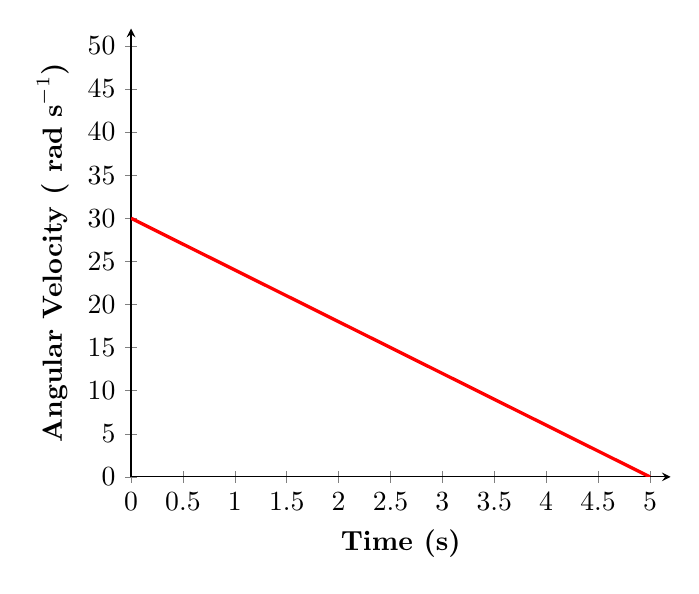
\begin{tikzpicture}
            \begin{axis}[
                axis lines=left,
                xlabel=\bf{Time (s)},
                ylabel=\bf{Angular Velocity ($\rads$)},
                xmax=5.2,
                ymax=52,
                xtick distance=0.5,
                ytick distance=5,
            ]
            \addplot[
                very thick,
                domain=0:5,
                samples=100,
                color=red,
                name path=A,
            ]
            {-6*x + 30};
                
            \end{axis}
        \end{tikzpicture}
    \end{center}
    \begin{enumerate}
        \item[(a)] Find the angular acceleration of the object and verify the result using kinematic equations
        \vspace{1mm}\\
        Because angular velocity varies linearly with time, angular acceleration is constant and not dependent on time. The angular acceleration is the derivative of angular velocity, $\alpha = \der{\omega}{t}$. At $t = 0$ s, $\omega_0 = 30\rads$ and at $t = 5$ s, $\omega_f = 0\rads$
        \begin{align*}
            \alpha = \frac{\omega - \omega_0}{t - t_0} = \frac{(0 - 30.0)\rads}{(5.0 - 0)\s} = -6.0\radss
        \end{align*}
        \item[(b)] Find the angle through which the propeller rotates during these 5 seconds and verify your result using kinematic equations
        \vspace{1mm}\\
        Since $\omega = \der{\theta}{t}$, angular displacement $\Delta\theta$ can be calculated by integrating the angular velocity
        \begin{align*}
            \int_{\theta_0}^{\theta_f}d\theta = \theta_f - \theta_0 = \int_{t_0}^{t_f}\omega(t)dt
        \end{align*}
        The area under the curve can be found by calculating the area of the right triangle shown:
        \begin{center}
            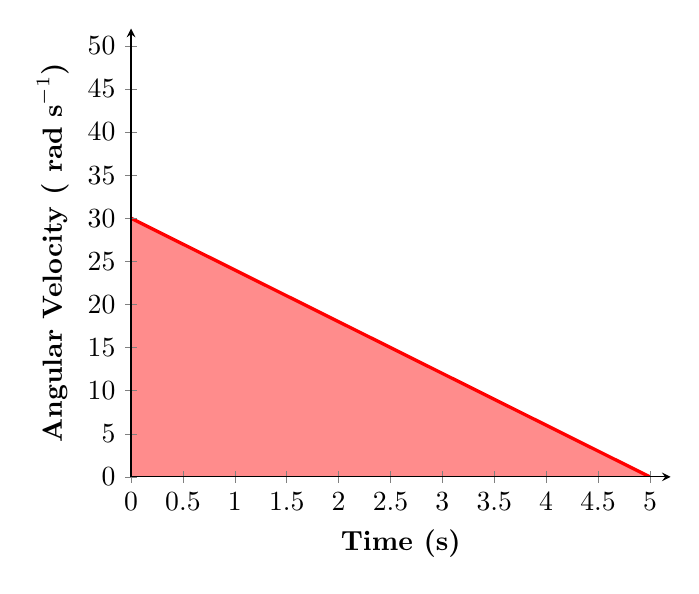
\begin{tikzpicture}
                \begin{axis}[
                    axis lines=left,
                    xlabel=\bf{Time (s)},
                    ylabel=\bf{Angular Velocity ($\rads$)},
                    xmax=5.2,
                    ymax=52,
                    xtick distance=0.5,
                    ytick distance=5,
                    axis on top,
                ]
                \addplot[
                    very thick,
                    domain=0:5,
                    samples=100,
                    color=red,
                    name path=A,
                ]
                {-6*x + 30};
                \path[name path=B]
                    (axis cs:\pgfkeysvalueof{/pgfplots/xmin},0)--
                    (axis cs:\pgfkeysvalueof{/pgfplots/xmax},0);
                \addplot[red!45] fill between[of=A and B,soft clip={domain=0:5},];
                \end{axis}
            \end{tikzpicture}
        \end{center}
        \begin{align*}
            \Delta\theta &= A(\text{triangle}) = \frac{1}{2}l \times h\\
            \Delta\theta &= \frac{1}{2}\Big(30\rads\Big)(5\s)
        \end{align*}
        This is verified using equation 12 ($\theta_f = \theta_0 + \omega_0t + \frac{1}{2}\alpha t^2$), and setting $\theta_0 = 0$ gives:
        \begin{align*}
            \theta_f = \big(30.0\rads\big)(5.0\s) + \frac{1}{2}\big(-6.0\radss\big)\big(5.0\rads\big)^2 = 150.0 - 75.0 = 75.0\rad
        \end{align*}
    \end{enumerate}
\end{shaded}

\subsection{Relating Angular and Translational Quantities}
\bf{Angular vs. Linear Variables}
\vspace{2mm}\\
Comparing the definitions of the rotational variables with the definitions of linear kinematic variables shows that there is a mapping of the linear variables to the rotational ones. Linear position, velocity, and acceleration have their rotational counterparts, as seen below.
\begin{center}
    \begin{tabularx}{0.4\textwidth}{ 
        | >{\raggedright\arraybackslash}X
        | >{\centering\arraybackslash}X  
        | >{\centering\arraybackslash}X |}
        \hline
        & \bf{Linear} & \bf{Rotational}\\
        \hline
        Position & $x$ & $\theta$\\
        \hline
        Velocity & $v = \der{x}{t}$ & $\omega = \der{\theta}{t}$\\
        \hline
        Acceleration & $a = \der{v}{t}$ & $\alpha = \der{\omega}{t}$\\
        \hline
    \end{tabularx}
\end{center}
In uniform and nonuniform circular motion, there exists a centripetal acceleration $a_c$. The centripetal acceleration vector points inward from the particle toward the axis of rotation. The magnitude of centripetal acceleration is:
\begin{equation}
    a_c = \frac{v^2_t}{r}
\end{equation}
In uniform circular motion, when $\omega =$ constant and $\alpha = 0$, there is a linear acceleration - centripetal acceleration - since $v_t =$ constant. If nonuniform circular motion is present, the rotating system has an angular acceleration, and there is both a linear centripetal acceleration that is changing ($\Delta v_t \neq 0$) as well as a linear tangential acceleration.
\begin{center}
    \begin{tikzpicture}[scale=1]
        \draw[thick] (0,0) circle (2cm);
        \draw[line width=0.5pt,dashed] (a)--(0,0);
        \draw ({2*cos(30)},{2*sin(30)}) coordinate (a);
        \draw (0,2) coordinate (b);
        \draw[->,very thick,-stealth,draw=blue] (a)--node[right]{$\vec{v}_1$}([turn]90:1.65cm);
        \draw[->,very thick,-stealth,draw=red] (a)--node[below]{$\vec{a}_c$}([turn]180:1.25cm);
        \draw[->,very thick,-stealth,draw=blue] (b)--node[above]{$\vec{v}_2$}([turn]90:1.65cm);
    \end{tikzpicture}
    \hspace{20mm}
    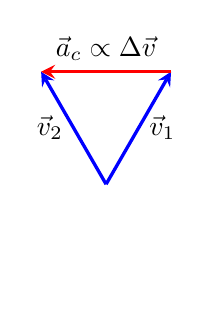
\begin{tikzpicture}[scale=1]
        \draw (0,0) coordinate (c);
        \draw (-{1.65*cos(60)},{1.65*sin(60)}) coordinate (a);
        \draw ({1.65*cos(60)},{1.65*sin(60)}) coordinate (b);
        \draw[->,very thick,-stealth,draw=blue] (c)--node[right]{$\vec{v}_1$}(b);
        \draw[->,very thick,-stealth,draw=blue] (c)--node[left]{$\vec{v}_2$}(a);
        \draw[->,very thick,-stealth,draw=red] (b)--node[above]{$\vec{a}_c \propto \Delta\vec{v}$}(a);
        \node at (0,-1.25){};
    \end{tikzpicture}
    \hspace{20mm}
    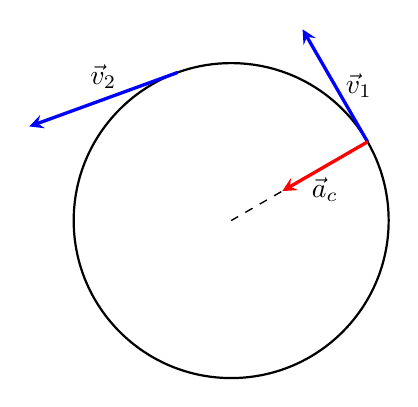
\begin{tikzpicture}[scale=1]
        \draw[thick] (0,0) circle (2cm);
        \draw[line width=0.5pt,dashed] ({2*cos(30)},{2*sin(30)})--(0,0);
        \draw ({2*cos(30)},{2*sin(30)}) coordinate (a);
        \draw ({-2*cos{70}},{2*sin(70)}) coordinate (b);
        \draw[->,very thick,-stealth,draw=blue] (a)--node[right]{$\vec{v}_1$}([turn]90:1.65cm);
        \draw[->,very thick,-stealth,draw=red] (a)--node[below]{$\vec{a}_c$}([turn]180:1.25cm);
        \draw[->,very thick,-stealth,draw=blue] (b)--node[above]{$\vec{v}_2$}([turn]90:2cm);
    \end{tikzpicture}
\end{center}
The centripetal acceleration is due to the change in the \underline{direction} of tangential velocity, whereas the tangential acceleration is due to any change in the \underline{magnitude} of the tangential velocity. The tangential and centripetal acceleration vectors $\vec{a}_t$ and $\vec{a}_c$ are always perpendicular to each other (the direction of $\vec{v}_t =$ the direction of $\vec{a}_t$).
\vspace{1mm}\\
We can assign a total linear acceleration vector to a point on a rotating rigid body or a particle executing circular motion at a radius $r$ from a fixed axis. The total linear acceleration vector $\vec{a}$ is the vector sum of the centripetal and tangential accelerations:
\begin{equation}
    \vec{a} = \vec{a}_c + \vec{a}_t
\end{equation}
The total linear acceleration vector in the case of nonuniform circular motion points at an angle between the centripetal and tangential acceleration vectors. Since $\vec{a}_c \perp \vec{a}_t$, the magnitude of the total linear acceleration is
\begin{align*}
    |\vec{a}| = \sqrt{a_c^2 + a_t^2}
\end{align*}
If the angular acceleration is zero, the total linear acceleration is equal to the centripetal acceleration
\begin{center}
    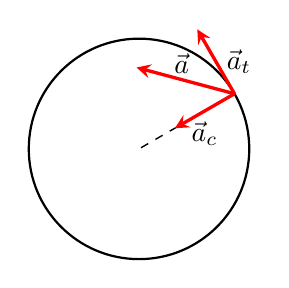
\begin{tikzpicture}[scale=0.7]
        \draw[thick] (0,0) circle (2cm);
        \draw[line width=0.5pt,dashed] ({2*cos(30)},{2*sin(30)})--(0,0);
        \draw ({2*cos(30)},{2*sin(30)}) coordinate (a);
        \draw ({-2*cos{70}},{2*sin(70)}) coordinate (b);
        \draw[->,very thick,-stealth,draw=red] (a)--node[right]{$\vec{a}_t$}([turn]90:1.35cm);
        \draw[->,very thick,-stealth,draw=red] (a)--node[below]{$\vec{a}_c$}([turn]180:1.25cm);
        \draw[->,very thick,-stealth,draw=red] (a)--node[above,xshift=-0.5mm,yshift=-0.5mm]{$\vec{a}$}([turn]135:1.84cm);
    \end{tikzpicture}
\end{center}

\noindent\bf{Relationship Between Rotational \& Translational Motion}
\vspace{2mm}\\
The relationship between the rotational and translational kinematic equations was mentioned above. The second relationship between rotational and translational motion relates linear and rotational variables in the special case of circular motion
\begin{center}
    \begin{tabularx}{0.4\textwidth}{ 
        | >{\raggedright\arraybackslash}X
        | >{\raggedright\arraybackslash}X  
        | >{\raggedright\arraybackslash}X |}
        \hline
        Rotational & Translational & Relationship\\[2.5pt]
        \hline
        $\theta$ & $s$ & $\theta = \frac{s}{r}$\\[2.5pt]
        \hline
        $\omega$ & $v_t$ & $\omega = \frac{v_t}{r}$\\[2.5pt]
        \hline
        $\alpha$ & $a_t$ & $\alpha = \frac{a_t}{r}$\\[2.5pt]
        \hline
        & $a_c$ & $a_c = \frac{v_t^2}{r}$\\[2.5pt]
        \hline
    \end{tabularx}
\end{center}

\newpage
\begin{shaded}
    \underline{\bf{Example 10.7} Linear Acceleration of a Centrifuge}
    \vspace{2mm}\\
    A centrifuge has a radius of 20 cm and accelerates from a maximum rotation rate of 10,000 rpm to rest in 30 seconds under a constant angular acceleration, rotating counterclockwise. What is the magnitude of the total acceleration for a point at the tip  of the centrifuge at $t = 29.0$ s? What is the direction of the total acceleration vector?
    \vspace{1mm}\\
    Angular acceleration is:
    \begin{align*}
        \alpha = \frac{\omega - \omega_0}{t} = \frac{0 - (1 \cdot 10^4)2\pi/60.0\s(\rads)}{30.0\s} = -34.9\radss
    \end{align*}
    Tangential acceleration is $a_t = r\alpha$, therefore:
    \begin{align*}
        a_t = 0.2\text{ m}(-34.9\radss) = -7.0\mss
    \end{align*}
    The angular velocity at $t = 29.0$ s can be found using the equation $\omega = \omega_0 + \alpha t$:
    \begin{align*}
        \omega &= \bigg[(1.0 \cdot 10^4\text{ rpm})\bigg(\frac{2\pi}{60\s}\bigg)\bigg]\rads + \big(-34.9\radss\big)(29.0\s)\\
        &= (1047.2 - 1012.71)\rads = 35.1\rads
    \end{align*}
    The tangential velocity $v_t$ is given by $v_t = r\omega$, therefore $v_t$ at $t = 29.0$ s is:
    \begin{align*}
        v_t = 0.2\m(35.1\rads) = 7.0\ms
    \end{align*}
    The centripetal acceleration $a_c$ at $t = 29.0\s$ can now be calculated using $a_c = \frac{v^2}{r}$, therefore:
    \begin{align*}
        a_c = \frac{(7.0\ms)^2}{0.2\m} = 245.0 \mss
    \end{align*}
    Since the two acceleration vectors are perpendicular to each other, the magnitude of the total linear acceleration is:
    \begin{align*}
        |\vec{a}| &= \sqrt{a_c^2 + a_t^2} = \sqrt{(245.0\mss)^2 + (-7.0\mss)^2}\\
        &= 245.1\mss
    \end{align*}
    Since the centrifuge has a negative angular acceleration, it is slowing down. The angle of the total acceleration vector with respect to the centripetal acceleration vector is:
    \begin{align*}
        \theta = \tan^{-1}\frac{-7.0\mss}{245.0\mss} = -1.6\degree
    \end{align*}
\end{shaded}
\newpage

\subsection{Moment of Inertia and Rotational Kinetic Energy}
This section introduces two new quantities that are helpful for analyzing properties of rotating objects: moment of inertia and rotational kinetic energy
\vspace{2mm}\\
\bf{Rotational Kinetic Energy}
\vspace{2mm}\\
The energy associated with rotational motion is the same as kinetic energy in translational motion however, because kinetic energy is given by $K = \frac{1}{2}mv^2$, and velocity is different for every point on a rotating body, it makes sense to write kinetic energy in terms of $\omega$. For a single particle rotating around a fixed axis, we relate the angular velocity to the magnitude of the translational velocity using the relation $v_t = \omega r$, where $r$ is the distance of the particle from the axis of rotation and $v_t$ is its tangential velocity. Substituting into the equation for kinetic energy gives:
\begin{align*}
    K = \frac{1}{2}mv_t^2 = \frac{1}{2}m(\omega r)^2 = \frac{1}{2}(mr^2)\omega^2
\end{align*}
In the case of a rigid rotating body, the total body can be divided up into a large number of smaller masses, each with mass $m_j$ and distance from the axis of rotation $r_j$, such that the total mass of the body $M$ is equal to the sum of the original masses $M = \sum_{j}m_j$. Each smaller mass has a tangential velocity $v_j$. The total kinetic energy of the rigid rotating body is:
\begin{align*}
    K = \sum_{j}\frac{1}{2}m_jv^2_j = \sum_{j}\frac{1}{2}m_j(r_j\omega_j)^2
\end{align*}
Since $\omega_j = \omega$ for all masses:
\begin{equation}
    K = \frac{1}{2}\bigg(\sum_{j}m_jr^2_j\bigg)\omega^2 
\end{equation}
Like translational kinetic energy, the units of this equation are joules (J)
\vspace{2mm}\\
\bf{Moment of Inertia}
\vspace{2mm}\\
The quantity $\sum\limits_j m_jr^2_j$ is the counterpart for mass in the equation for rotational kinetic energy. This quantity is called the moment of inertia $I$ and has units of$\kgmm$
\begin{equation}
    I = \sum_{j}m_jr^2_j
\end{equation}
For now the expression is left in summation form, representing the moment of inertia of a system of point particles rotating about a fixed axis. The moment of inertia of a single point particle about a fixed axis is simply $mr^2$.
\vspace{1mm}\\
The moment of inertia is the quantitative measure of rotational inertia, just as in translational motion, mass is the quantitative measure of linear inertia - that is, the more massive an object is, the more inertia it has, and the greater is its resistance to change in linear velocity. Similarly, the greater the moment of inertia of a rigid body or system of particles, the greater its resistance to change in angular velocity about a fixed axis of rotation. Rigid bodies and systems of particles with more mass concentrated at a greater distance from the axis of rotation have greater moments of inertia than bodies/systems of the same mass bt concentrated near the axis of rotation. Substituting equation 17 into equation 16, the expression for the kinetic energy of a rotating rigid body becomes:
\begin{equation}
    K = \frac{1}{2}I\omega^2
\end{equation}
The kinetic energy of a rotating rigid body is directly proportional to the moment of inertia and the square of the angular velocity. The rotational and translational quantities for kinetic energy are summarized below:
\begin{center}
    \begin{tabularx}{0.4\textwidth}{ 
        | >{\raggedright\arraybackslash}X 
        | >{\raggedright\arraybackslash}X |}
        \hline
        Rotational & Translational\\
        \hline
        $\displaystyle I = \sum_{j}m_jr^2_j$ & $m$\\
        \hline
        $\displaystyle K = \frac{1}{2}I\omega^2$ & $\displaystyle K = \frac{1}{2}mv^2$\\
        \hline
    \end{tabularx}
\end{center}

\newpage
\begin{shaded}
    \underline{\bf{Example 10.8:} Moment of Inertia of a System of Particles}
    \vspace{2mm}\\
    Six small washers are spaced 10 cm apart on a rod of negligible mass and 0.5 m in length. The mass of each washer is 20 g. The rod rotates about an axis located at 25 cm as shown.
    \begin{center}
        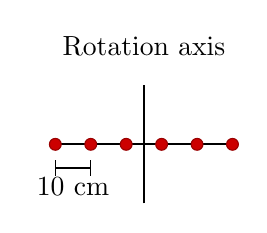
\begin{tikzpicture}[scale=1.5]
            \draw[line width=0.5pt] (0,-0.5)--(0,0.5);
            \draw[-,thick] (-0.75,0)--(0.75,0);
            \filldraw[draw=black!40!red,fill=black!20!red] (-0.75,0) circle (0.05);
            \filldraw[draw=black!40!red,fill=black!20!red] (-0.45,0) circle (0.05);
            \filldraw[draw=black!40!red,fill=black!20!red] (0.75,0) circle (0.05);
            \filldraw[draw=black!40!red,fill=black!20!red] (0.45,0) circle (0.05);
            \filldraw[draw=black!40!red,fill=black!20!red] (0.15,0) circle (0.05);
            \filldraw[draw=black!40!red,fill=black!20!red] (-0.15,0) circle (0.05);
            \draw[|-|] (-0.75,-0.2)--node[below]{10 cm}(-0.45,-0.2);
            \centerarc[->,thick,draw=black,-stealth](0,0.5)(120:210:0.1667);
            \centerarc[->,thick,draw=black,-stealth](0,0.5)(350:420:0.1667);
            \centerarc[->,thick,draw=black,-stealth](0,0.5)(210:350:0.1667);
            \node[above,yshift=1mm] at (0,0.6){Rotation axis};
        \end{tikzpicture}
    \end{center}
    \begin{enumerate}
        \item[(a)] What is the moment of inertia of the system?
        \vspace{1mm}\\
        Use the definition of moment of inertia for a system of particles: $I = \sum\limits_j m_jr^2_j$
        \begin{align*}
            I &= (0.02\kg)\big[2(0.25\m)^2 + 2(0.15\m)^2 + 2(0.05\m)^2\big]\\
            &= 3.5 \cdot 10^{-3}\kgmm
        \end{align*}
        \item[(b)] If the two washers closest to the axis are removed, what is the moment of inertia of the remaining four washers?
        \vspace{1mm}\\
        Repeat the steps from part (a):
        \begin{align*}
            I &= (0.02\kg)\big[2(0.25\m)^2 + 2(0.15\m)^2\big]\\
            &= 3.4 \cdot 10^{-3}\kgmm
        \end{align*}
        \item[(c)] If the system with six washers rotates at 5 rev/s, what is its rotational kinetic energy?
        \vspace{1mm}\\
        Insert the result from part (a) into the expression for rotational kinetic energy:
        \begin{align*}
            K &= \frac{1}{2}I\omega^2\\
            &= \frac{1}{2}(3.5 \times 10^{-3}\kgmm)\big[5.0(2\pi\rads)\big]^2\\
            &= 1.73\J
        \end{align*}
    \end{enumerate}
\end{shaded}
\newpage
\noindent\bf{Applying Rotational Kinetic Energy}
\begin{shaded}
    \underline{\bf{Problem Solving Strategy:} Rotational Energy}
    \begin{enumerate}
        \item Determine that energy or work is involved in the rotation
        \item Determine the system of interest
        \item Analyze the situation to determine the types of work and energy involved
        \item If there are no losses of energy due to friction and other nonconservative forces, mechanical energy is conserved: $K_0 + U_0 = K_f + U_f$
        \item If nonconservative forces are present, mechanical energy is not conserved, determine what they are and calculate them as necessary
        \item Eliminate terms wherever possible to simplify the algebra
        \item Evaluate the numerical solution to see if it makes sense in the physical situation presented in the wording of the problem
    \end{enumerate}
\end{shaded}

\begin{shaded}
    \underline{\bf{Example 10.9:} Calculating Helicopter Energies}
    \vspace{2mm}\\
    A typical small rescue helicopter has four blades, each is 4.00 m long and has a mass of 50.0 kg. The blades can be approximated as thin rods that rotate about one end of an axis perpendicular to their length. The helicopter has a total loaded mass of 1000 kg.
    \begin{enumerate}
        \item[(a)] Calculate the rotational kinetic energy in the blades when they rotate at 300 rpm
        \vspace{2mm}\\
        The rotational kinetic energy is given by $\frac{1}{2}I\omega^2$. First, the angular velocity must be converted to$\rads$, the angular velocity $\omega$ is
        \begin{align*}
            \omega = \frac{300\text{ rev}}{1.00\text{ min}} \cdot \frac{2\pi\rad}{1\text{ rev}} \cdot \frac{1.00\text{ min}}{60.0\s} = 31.4\rads
        \end{align*}
        The moment of inertia of one blade is that of a thin rod rotated about its end, the total $I$ is 4 times this because there are 4 blades.
        \begin{align*}
            I = 4\frac{ML^2}{3} = 4\bigg(\frac{(50.0\kg)(4.00\m)^2}{3}\bigg) = 1067.0\kgmm
        \end{align*}
        Entering $\omega$ and $I$ into the expression for rotational kinetic energy gives:
        \begin{align*}
            K &= \frac{1}{2}I\omega^2\\
            &= \frac{1}{2}(1067\kgmm)(31.4\rads)^2\\
            &= 5.26 \cdot 10^5\J
        \end{align*}
        \item[(b)] Calculate the translational kinetic energy of the helicopter when it flies at 20.0$\ms$, and compare it with the rotational energy in the blades
        \vspace{1mm}\\
        Entering the given values into the equation for translational kinetic energy gives:
        \begin{align*}
            K &= \frac{1}{2}mv^2\\
            &= \frac{1}{2}(10^3\kg)(20\ms)^2\\
            &= 2.00 \cdot 10^5\J
        \end{align*}
        To compare kinetic energies take the ratio of translational kinetic energy to rotational kinetic energy:
        \begin{align*}
            \frac{2.00 \cdot 10^5\J}{5.26 \cdot 10^5\J} = 0.380
        \end{align*}
        This tells us that most of the energy of the helicopter is in its spinning blades
    \end{enumerate}
\end{shaded}

\begin{shaded}
    \underline{\bf{Example 10.10:} Energy in a Boomerang}
    \vspace{2mm}\\
    A person hurls a boomerang into the air with a velocity of 30.0$ms$ at an angle of 40.0$\degree$ with respect to the horizontal. It has a mass of 1.0 kg and it rotating at 10.0 rev/s. The moment of inertia of the boomerang is given as $I = \frac{1}{12}mL^2$ where $L = 0.7\m$. 
    \begin{enumerate}
        \item[(a)] What is the total energy of the boomerang when it leaves the hand?
        \vspace{1mm}\\
        The total kinetic energy of the boomerang is: $K_{tot} = K_R + K_T$\\
        The moment of inertia is: $\displaystyle I = \frac{1}{12}mL^2 = \frac{1}{12}(1.0\kg)(0.7\m)^2 = 0.041\kgmm$\\
        The angular velocity is: $\omega = 2\pi(10.0\text{ rev/s}) = 62.83\rads$\\
        Therefore the rotational and translational kinetic energies are:\\
        \begin{minipage}{0.4\textwidth}
            \begin{align*}
                K_R &= \frac{1}{2}I\omega^2\\
                &= \frac{1}{2}(0.041\kgmm)(62.83\rads)^2\\
                &= 80.93\J
            \end{align*}            
        \end{minipage}
        \begin{minipage}{0.4\textwidth}
            \begin{align*}
                K_T &= \frac{1}{2}mv^2\\
                &= \frac{1}{2}(1.0\kg)(30.0\ms)^2\\
                &= 450.0\J
            \end{align*}
        \end{minipage}\\
        Therefore, the total kinetic energy of the boomerang is $\displaystyle K_{tot} = (80.93 + 450.0)\J = 530.93\J$
        \item[(b)] How high does the boomerang go from the elevation of the hand, neglecting air resistance?
        \vspace{1mm}\\
        The maximum height can be found using the conservation of mechanical energy ($E_0 = E_f$). Since the boomerang is launched at an angle, the total energy of the system must be written in terms of its linear kinetic energies using velocity in the $x$ and $y$ directions.\\
        The energy when the boomerang leaves the hand is: $\displaystyle E_0 = \frac{1}{2}mv_x^2 + \frac{1}{2}mv_y^2 + \frac{1}{2}I\omega^2$\\
        The total energy at the maximum height $h$ is: $\displaystyle E_f = \frac{1}{2}mv_x^2 + \frac{1}{2}I\omega^2 + mgh$\\
        Equating and canceling like terms gives:
        \begin{align*}
            \cancel{\frac{1}{2}mv_x^2} + \frac{1}{2}mv_y^2 + \cancel{\frac{1}{2}I\omega^2} &= \cancel{\frac{1}{2}mv_x^2} + \cancel{\frac{1}{2}I\omega^2} + mgh\\
            \frac{1}{2}mv_y^2 &= mgh
        \end{align*}
        Rearranging and entering known values gives:
        \begin{align*}
            h &= \frac{\cancel{m}v_y^2}{2\cancel{m}g} \to h = \frac{v_y^2}{2g}\\
            h &= \frac{(19.28\ms)^2}{2(9.8\mss)} = 18.97\m
        \end{align*}
    \end{enumerate} 
\end{shaded}
\newpage

\subsection{Calculating Moments of Inertia}
This section covers how to calculate the moment of inertia for several standard types of objects, as well as how to use known moments of inertia to find the moment of inertia for a shifted axis or for a compound object.
\vspace{2mm}\\
\bf{Moment of Inertia}
\vspace{1mm}\\
The moment of inertia $I$ of an object is defined to be $I = \sum\limits_{i}m_ir^2_i$ for all the point masses that make up the object. Because $r$ is the distance to the axis of rotation for each piece of mass that makes up the object, the moment of inertia depends on the chosen axis. Take a simple example of two masses at the end of a massless (negligibly small mass) rod and calculate the moment of inertia about two different axes. The summation over the masses is simple because the two masses can be approximated as point masses, and the sum has only two terms.\vspace{1mm}\\
In the case with the axis in the center of the barbell, each of the two masses $m$ is a distance $R$ away from the axis giving a moment of inertia of
\begin{align*}
    I_1 = mR^2 + mR^2 = 2mR^2
\end{align*}
In the case with the axis at the end of the barbell (passing through one of the masses) the moment of inertia is:
\begin{align*}
    I_2 = m(0)^2 + m(2R)^2 = 4mR^2
\end{align*}
From this result we can conclude that it is twice as hard to rotate the barbell about the end than about its center.\vspace{1mm}\\
%%% Add figure?? %%%
This example uses two point masses, making the sum easy to calculate. In the derivation of equation 17, each piece had the same magnitude of velocity, meaning the whole piece had to have a single distance $r$ to the axis of rotation. This is only possible taking an infinitesimally small piece of mass $dm$. This suggests that the moment of inertia can be written by evaluating an integral over infinitesimal masses rather than doing a discrete sum over finite masses:
\begin{equation}
    I = \sum_{i}m_ir_i^2\ \boldsymbol{\to}\ I = \int r^2dm
\end{equation}
This is all that is needed to generalize the equation for complex chapes
\vspace{2mm}\\
\bf{A Uniform Thin Rod With an Axis Through The Center}
\vspace{2mm}\\
Consider a uniform ($\rho$ \& shape) thin rod of mass $M$ and length $L$ as shown. We want a thin rod so that we can assume the cross-sectional area of the rod is small and the rod can be thought of as a string of masses along a 1D straight line. In this example, the axis of rotation is perpendicular to the rod and passes through the midpoint. The axes are oriented so that the $z$ axis is the axis of rotation and the $x$ axis passes through the length of the rod.
\begin{center}
    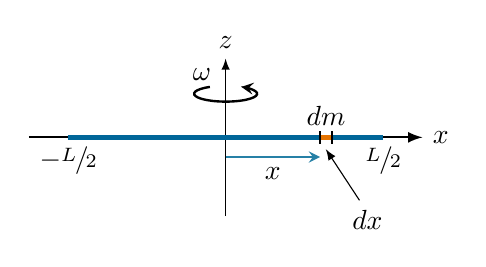
\begin{tikzpicture}[scale=2]
        \draw[->,thick,-latex] (-1.25,0)--(1.25,0) node[right]{$x$};
        \draw[->,-latex] (0,-0.5)--node[above,yshift=3mm]{\AxisRotator[x=0.1cm,y=0.4cm,rotate=-90]}(0,0.5) node[above]{$z$};
        \node[above] at (-0.15,0.3){$\omega$};
        \draw[line width=1.75pt,draw=green!40!blue] (-1,0)--(1,0);
        \draw[line width=1.75pt,draw=black!10!orange] (0.6,0)--node[above]{$dm$}(0.675,0);
        \node[below] at (-1,0){$-\sfrac{L}{2}$};
        \node[below] at (1,0){$\sfrac{L}{2}$};
        \draw[line width=0.5pt] (0.6,0.04)--(0.6,-0.04);
        \draw[line width=0.5pt] (0.675,0.04)--(0.675,-0.04);
        \draw[->,-stealth,thick,draw=white!30!green!50!blue] (0,-0.125)--node[below]{$x$}(0.6,-0.125);
        \draw[->,-latex] (0.85,-0.4)--(0.63625,-0.075);
        \node[below,xshift=1mm] at (0.85,-0.4){$dx$};
    \end{tikzpicture}
\end{center}
We define $dm$ to be a small element of the mass making up the rod. The moment of inertia integral is an integral over the mass distribution. However, we know how to integrate over space, not mass and therefore need to find a way to relate mass to spatial variables. This is done using the linear mass density $\lambda$ of the object, which is the mass per unit length. Since the mass and density of the object are both uniform:
\begin{align*}
    \lambda = \frac{m}{L}\ \boldsymbol{\to}\ m = \lambda L
\end{align*}
Since $\lambda$ is constant, taking the differential of each side of the equation gives:
\begin{align*}
    dm = d(\lambda L) = \lambda(dL)
\end{align*}
This is where the choice to orient the rod along the $x$ axis becomes helpful. A piece of the rod $dl$ lies completely along the $x$ axis and has a length $dx$, in this situation $dL = dx$. Therefore $dm = \lambda(dx)$, giving an integration variable that can be used. The distance of each piece of mass $dm$ from the axis is given by the variable $x$, putting this all together gives:
\begin{align*}
    I = \int r^2dm = \int x^2dm = \int x^2\lambda dx 
\end{align*}
The last step is to be careful about the limits of integration. The rod extends from $x = -\sfrac{L}{2}$ to $x = \sfrac{L}{2}$, since the axis is in the middle of the rod at $x = 0$. This gives:
\begin{align*}
    I &= \int\limits_{-\sfrac{L}{2}}^{\sfrac{L}{2}} x^2\lambda dx = \lambda\frac{x^3}{3}\Bigg\vert_{-\sfrac{L}{2}}^{\sfrac{L}{2}} = \lambda\bigg(\frac{1}{3}\bigg)\Bigg[\bigg(\frac{L}{2}\bigg)^3 - \bigg(-\frac{L}{2}\bigg)^3\Bigg]\\
    &= \lambda\bigg(\frac{1}{3}\bigg)\frac{L^3}{8}(2) = \frac{M}{L}\bigg(\frac{1}{3}\bigg)\frac{L^3}{8}(2) = \frac{1}{12}ML^2
\end{align*}
\newpage
\noindent\bf{A Uniform Thin Rod With Axis at The End}
\vspace{2mm}\\
Now consider the same uniform thin rod of mass $M$ and length $L$ this time with the axis of rotation at the end of the rod. The quantity $dm$ is again defined to be a small element of mass making up the rod, just as before:
\begin{align*}
    I = \int r^2dm = \int x^2dm = \int x^2\lambda dx
\end{align*}
However, this time there are different limits of integration. The rod extends from $x = 0$ to $x = L$, since the axis is at the end of the rod at $x = 0$. Therefore:
\begin{align*}
    I &= \int_{0}^{L}x^2\lambda dx = \lambda\frac{x^3}{3} \Bigg\vert_0^L = \lambda \bigg(\frac{1}{3}\bigg)\Big[(L)^3 - (0)^3\Big]\\
    &= \lambda\bigg(\frac{1}{3}\bigg)L^3 = \frac{M}{L}\bigg(\frac{1}{3}\bigg)L^3 = \frac{1}{3}ML^2
\end{align*}
Note that the rotational inertia of the rod about its endpoint is larger than the rotational inertia about its center by a factor of four.
\begin{center}
    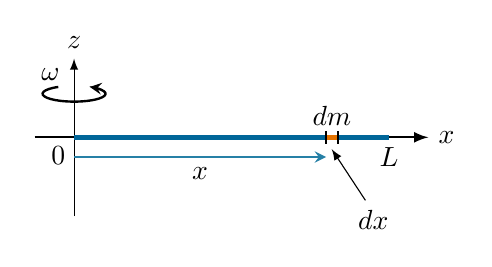
\begin{tikzpicture}[scale=2]
        \draw[->,thick,-latex] (-1.25,0)--(1.25,0) node[right]{$x$};
        \draw[->,-latex] (-1,-0.5)--node[above,yshift=3mm]{\AxisRotator[x=0.1cm,y=0.4cm,rotate=-90]} (-1,0.5) node[above]{$z$};
        \node[above] at (-1.15,0.3){$\omega$};
        \draw[line width=1.75pt,draw=green!40!blue] (-1,0)--(1,0);
        \draw[line width=1.75pt,draw=black!10!orange] (0.6,0)--node[above]{$dm$}(0.675,0);
        \node[below] at (-1.1,0){$0$};
        \node[below] at (1,0){$L$};
        \draw[line width=0.5pt] (0.6,0.04)--(0.6,-0.04);
        \draw[line width=0.5pt] (0.675,0.04)--(0.675,-0.04);
        \draw[->,-stealth,thick,draw=white!30!green!50!blue] (-1,-0.125)--node[below]{$x$}(0.6,-0.125);
        \draw[->,-latex] (0.85,-0.4)--(0.63625,-0.075);
        \node[below,xshift=1mm] at (0.85,-0.4){$dx$};
    \end{tikzpicture}
\end{center}
\bf{Parallel-Axis Theorem}
\vspace{2mm}\\
The parallel-axis theorem provides a simpler method for determining the moment of inertia for a rod about any axis parallel to the axis through the center of mass.
\vspace{1mm}\\
Let $m$ be the mass of an object and let $d$ be the distance from an axis through the object's center of mass to a new axis:
\begin{equation}
    I_{pa} = I_{cm} + md^2
\end{equation}
Applying this to the examples solved above:
\begin{align*}
    I_{end} = I_{cm} + md^2 = \frac{1}{12}mL^2 + m\bigg(\frac{L}{2}\bigg)^2 = \bigg(\frac{1}{12} + \frac{1}{4}\bigg)mL^2 = \frac{1}{3}mL^2
\end{align*}
This result agrees with the more lengthy calculation above.
\vspace{2mm}\\
\bf{A Uniform Thin Disk About an Axis Through The Center}
\vspace{2mm}\\
Integrating to find the moment of inertia of a 2D object is a little bit trickier however, one shape is commonly done at this level of study, a uniform thin disk about an axis through its center
\begin{center}
    \begin{minipage}{0.4\textwidth}
        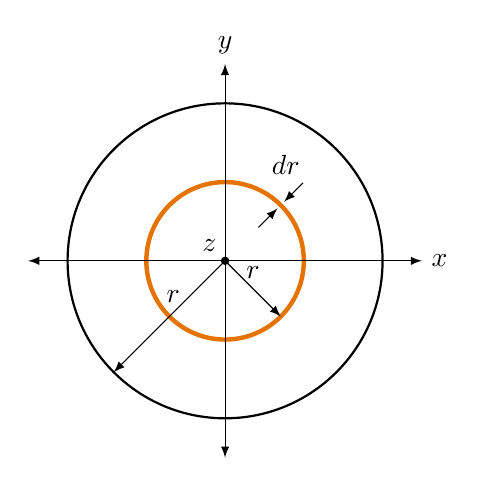
\begin{tikzpicture}[scale=2]
            \draw[thick] (0,0) circle (1);
            \draw[ultra thick,draw=black!10!orange] (0,0) circle (0.5);
            \filldraw[black] (0,0) circle (0.65pt);
            \node at (-0.1,0.1){$z$};
    
            \draw[<->,latex-latex] (-1.25,0)--(1.25,0) node[right]{$x$};
            \draw[<->,latex-latex] (0,-1.25)--(0,1.25) node[above]{$y$};
    
            \draw[->,-latex] (0,0)--node[above,yshift=0.5mm,xshift=0.5mm]{$r$}(-{cos(45)},-{sin(45)});
            \draw[->,-latex] (0,0)--node[above]{$r$}({0.5*cos(45)},-{0.5*sin(45)});
    
            \draw[->,-latex] ({0.3*cos(45)},{0.3*sin(45)})--({0.47*cos(45)},{0.47*sin(45)});
            \draw[->,-latex] ({0.7*cos(45)},{0.7*sin(45)})--node[above,xshift=-1mm,yshift=1mm]{$dr$}({0.53*cos(45)},{0.53*sin(45)});
        \end{tikzpicture}
    \end{minipage}
    \begin{minipage}{0.4\textwidth}
        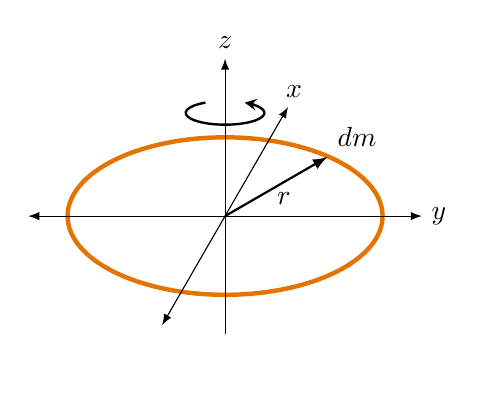
\begin{tikzpicture}[scale=2]
            \draw[ultra thick,draw=black!10!orange] (0,0) ellipse (1 and 0.5);
            
            \draw[<->,latex-latex] (-1.25,0)--(1.25,0) node[right]{$y$};
            \draw[->,-latex] (0,-0.75)--(0,1) node[above,yshift=-1cm]{\AxisRotator[x=0.15cm,y=0.5cm,rotate=-90]} node[above]{$z$};
            \draw[<->,latex-latex] ({-0.8*cos(60)},{-0.8*sin(60)})--({0.8*cos(60)},{0.8*sin(60)}) node[above,xshift=0.75mm]{$x$};

            \draw[->,thick,-latex] (0,0)--node[below,xshift=1mm,yshift=0.5mm]{$r$}({0.75*cos(30)},{0.75*sin(30)}) node[right,yshift=2.5mm]{$dm$};
            \node at (0,-1){};
        \end{tikzpicture}        
    \end{minipage}
\end{center}
Since the disk is think, we can take the mass as distributed entirely in the $xy$ plane. Starting again with the relationship for the surface mass density, which is the mass per unit surface area. Since it is uniform, the surface mass density $\sigma$ is constant:
\begin{align*}
    \sigma = \frac{m}{A} \to \sigma A = m\text{, so: } dm = \sigma(dA)
\end{align*}
Now we use a simplification for the area. The area can be thought of as made up of a series of thin rings, where each ring is a mass increment $dm$ of radius $r$ equidistant from the axis. The infinitesimal area of each ring $dA$ is therefore given by the length of each ring ($2\pi r$) times the infinitesimal width of each ring $dr$:
\begin{align*}
    A = \pi r^2,\ dA = d(\pi r^2) = \pi dr^2 = 2\pi rdr
\end{align*}
\newpage\noindent
The full area of the disk is then made up from adding all the thin rings with a radius range from 0 to $R$. This radius range then becomes our limits of integration for $dr$, we integrate from $r = 0$ to $r = R$. Putting this together gives:
\begin{align*}
    I &= \int_{0}^{R} r^2\sigma(2\pi r)dr = 2\pi\sigma\int_{0}^{R}r^3dr = 2\pi\sigma\frac{r^4}{4}\Bigg\vert_0^R = 2\pi\sigma\bigg(\frac{R^4}{4} - 0\bigg)\\
    &= 2\pi\frac{m}{A}\bigg(\frac{R^4}{4}\bigg) = 2\pi\frac{m}{\pi R^2}\bigg(\frac{R^4}{4}\bigg) = \frac{1}{2}mR^2
\end{align*}
\vspace{2mm}\\
\bf{Calculating The Moment of Inertia For Compound Objects}\vspace{2mm}\\
Now consider a compound object like a disk at the end of a thin rod. This cannot be easily integrated to find the moment of inertia because it is not a uniformly shaped object. However, going back to the initial definition of moment of inertia as a summation, we can reason that a compound object's moment of inertia can be found from the sum of each part of the object:
\begin{equation}
    I_{tot} = \sum_{i} I_i
\end{equation}
It is important to note that the moments of inertia of the objects in equation 21 are about a common axis. In the case of this object, that would be a rod of length $L$ rotating about its end, and a thin disk of radius $R$ rotating about an axis shifted off the center by a distance $L + R$, where $R$ is the radius of the disk. We define the mass of the rod to be $m_r$ and the mass of the disk to be $m_d$
\begin{center}
    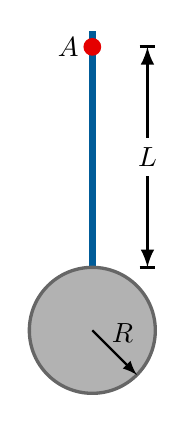
\begin{tikzpicture}[scale=2]
        \draw[line width=2.5pt,draw=black!10!green!40!blue] (0,0)--(0,1.5);
        \filldraw[black!30] (0,-0.4) circle(0.4);
        \draw[black!60,very thick] (0,-0.4) circle (0.4);
        \draw[->,thick,-latex] (0,-0.4)--node[above,xshift=1mm]{$R$}({0.4*cos(45)},{-0.4*sin(45) - 0.4});
        \filldraw[black!10!red] (0,1.4) circle (1.5pt) node[text=black,left,xshift=-0.5mm]{$A$};
        \draw[<->,very thick,latex-latex] (0.35,0)--node[fill=white]{$L$}(0.35,1.4);
        \draw[line width=1pt] (0.3,0)--(0.4,0);
        \draw[line width=1pt] (0.3,1.4)--(0.4,1.4);
    \end{tikzpicture}
\end{center}
The moment of inertia of the rod is simply $\frac{1}{3}m_rL^2$, but to find the moment of inertia of the disk about the axis shown, parallel-axis theorem must be used. The moment of inertia of the disk about its center ia $\frac{1}{2}m_dR^2$, applying the parallel-axis theorem $I_{pa} = I_{cm} + md^2$ to find
\begin{align*}
    I_{pa} = \frac{1}{2}m_dR^2 + m_d(L + R)^2
\end{align*}
\bf{Applying Moment of Inertia Calculations to Solve Problems}
\begin{shaded}
    \underline{\bf{Example 10.11:} Person on a Merry-Go-Round}
    \vspace{2mm}\\
    A 25 kg child stands a distance $r = 1.0\m$ from the axis of a rotating merry-go-round. The merry-go-round can be approximated as a uniform solid disk with a mass of 500 kg and radius of 2.0 m. Find the moment of inertia of the system
    \vspace{1mm}\\
    The mass and distance to the axis of rotation of the child as well as the mass and radius of the merry-go-round are given. Since the mass and size of the child are much smaller than the merry-go-round, we can approximate the child as a point mass\\
    $m_c = 25\kg,\ r_c = 1.0\m,\ m_m = 500\kg,\ r_m = 2.0\m,\ $ The goal is to find $\sum\limits_{i}I_i$
    \vspace{1mm}\\
    For the child, $I_c = m_cr^2$, and for the merry-go-round, $I_m = \frac{1}{2}m_mr^2$, therefore
    \begin{align*}
        I_{tot} &= I_c + I_m\\
        &= 25(1)^2 + \frac{1}{2}(500)(2)^2 = 25 + 1000\\
        &= 1025\kg
    \end{align*}
    The value should be close to the moment of inertia of the merry-go-round by itself because it has much more mass distributed away from the axis than the child does.
\end{shaded}

\begin{shaded}
    \underline{\bf{Example 10.12:} Rod and Solid Sphere}
    \vspace{2mm}\\
    Find the moment of inertia of the rod and solid sphere combination about the two axes as shown below. The rod has a length of 0.5 m and a mass of 2.0 kg. The radius of the sphere is 20.0 cm and has a mass of 1.0 kg.
    \begin{center}
        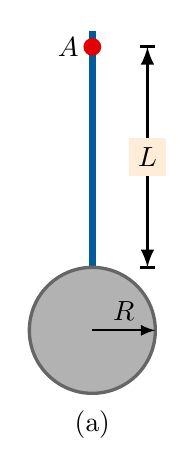
\begin{tikzpicture}[scale=2]
            \draw[line width=2.5pt,draw=black!10!green!40!blue] (0,0)--(0,1.5);
            \filldraw[black!30] (0,-0.4) circle(0.4);
            \draw[black!60,very thick] (0,-0.4) circle (0.4);
            \draw[->,thick,-latex] (0,-0.4)--node[above]{$R$}(0.4,-0.4);
            \filldraw[black!10!red] (0,1.4) circle (1.5pt) node[text=black,left,xshift=-0.5mm]{$A$};
            \draw[<->,very thick,latex-latex] (0.35,0)--node[fill=orange!15]{$L$}(0.35,1.4);
            \draw[line width=1pt] (0.3,0)--(0.4,0);
            \draw[line width=1pt] (0.3,1.4)--(0.4,1.4);
            \node at (0,-1){(a)};
        \end{tikzpicture}
        \hspace{5cm}
        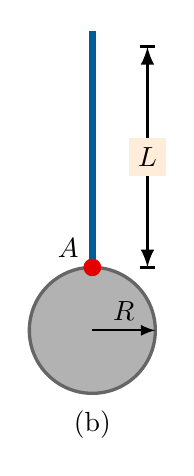
\begin{tikzpicture}[scale=2]
            \draw[line width=2.5pt,draw=black!10!green!40!blue] (0,0)--(0,1.5);
            \filldraw[black!30] (0,-0.4) circle(0.4);
            \draw[black!60,very thick] (0,-0.4) circle (0.4);
            \draw[->,thick,-latex] (0,-0.4)--node[above]{$R$}(0.4,-0.4);
            \filldraw[black!10!red] (0,0) circle (1.5pt) node[text=black,left,yshift=2.5mm,xshift=-0.5mm]{$A$};
            \draw[<->,very thick,latex-latex] (0.35,0)--node[fill=orange!15]{$L$}(0.35,1.4);
            \draw[line width=1pt] (0.3,0)--(0.4,0);
            \draw[line width=1pt] (0.3,1.4)--(0.4,1.4);
            \node at (0,-1){(b)};
        \end{tikzpicture}
    \end{center}
    In (a), the center of mass of the sphere is located a distance $L + R$ from the axis of rotation. In (b), the center of mass is located a distance $R$ from the axis of rotation. In both cases, the moment of inertia of the rod is about an axis at one end.
    \begin{enumerate}
        \item For axis (a), the moment of inertia is:
        \begin{align*}
            I_{tot} &= \sum_{i}I_i = I_r + I_s\\
            I_s &= I_{cm} + m_s(L + R)^2 = \frac{2}{5}m_sR^2 + m_s(L + R)^2\\
            I_{tot} &= I_r + I_s = \frac{1}{3}m_rL^2 + \frac{2}{5}m_sR^2 + m_s(L + R)^2\\
            &= \frac{1}{3}(2.0\kg)(0.5\m)^2 + \frac{2}{5}(1.0\kg)(0.2\m)^2 + (1.0\kg)(0.5\m + 0.2\m)^2\\
            &= (0.167 + 0.016 + 0.490)\kgmm = 0.673\kgmm
        \end{align*}
        \item[(b)] For axis (b), the moment of inertia is:
        \begin{align*}
            I_s &= \frac{2}{5}m_sR^2 + m_sR^2\\
            I_{tot} &= I_r + I_s = \frac{1}{3}m_rL^2 + \frac{2}{5}m_sR^2 + m_sR^2\\
            &= \frac{1}{3}(2.0\kg)(0.5\m)^2 + \frac{7}{5}(1.0\kg)(0.2\m)^2\\
            &= (0.167 + 0.056)\kgmm = 0.223\kgmm
        \end{align*}
    \end{enumerate}
\end{shaded}

\newpage
\begin{shaded}
    \underline{\bf{Example 10.13:} Angular Velocity of a Pendulum}
    \vspace{2mm}\\
    A pendulum in the shape of a rod is released from rest at an angle of $30\degree$. It has a length of 30 cm and a mass of 300 g. What is its angular velocity $\omega$ at its lowest point?
    \begin{center}
        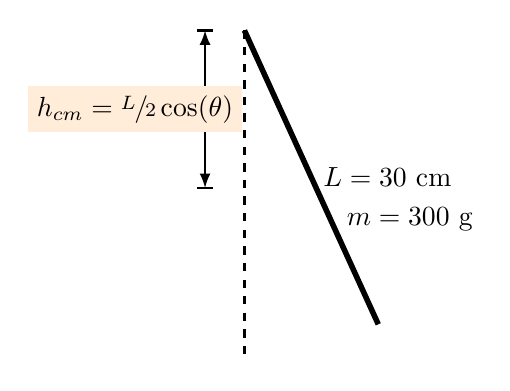
\begin{tikzpicture}[scale=2]
            \draw[line width=1pt,dashed] (0,1)--(0,-1.1);
            \draw[<->,thick,latex-latex] (-0.25,0)--node[fill=orange!15,xshift=-8.9mm]{$h_{cm} = \sfrac{L}{2}\cos(\theta)$} (-0.25,1);
            \draw[line width=1pt] (-0.3,0)--(-0.2,0);
            \draw[line width=1pt] (-0.3,1)--(-0.2,1);
            \draw[line width=2pt] (0,1)--node[right]{$L = 30$ cm}({1.7*cos(60)},{ -1*sin(60)});
            \node at (1.05,-0.2){$m = 300$ g};
            \centerarc[<-,red,very thick,latex-](0,1)(289:300:2.1);
        \end{tikzpicture}
    \end{center}
    Use conservation of energy to solve the problem. At the point of release, the pendulum has gravitational potential energy which is determined from the height of the center of mass above the lowest point in the swing. At the bottom of the swing, all of the gravitational potential energy is converted into rotational kinetic energy.
    \vspace{1mm}\\
    The change in Potential energy is equal to the change in rotational kinetic energy, $\Delta U + \Delta K = 0$\\
    At the top of the swing, $\displaystyle U = mgh_{cm} = mg\frac{L}{2}$. At the bottom of the swing, $\displaystyle U = mg\frac{L}{2}$ with respect to the lowest point\\
    At the top of the swing, the rotational kinetic energy is $K = 0$. At the bottom of the swing $K = \frac{1}{2}I\omega^2$, therefore:
    \begin{align*}
        \Delta U + \Delta K = 0\ \boldsymbol{\to}\ \Big(mg\frac{L}{2}\big(1 - \cos(\theta)\big) - 0\Big) + \Big(0 - \frac{1}{2}I\omega^2\Big) = 0
    \end{align*}
    Or,
    \begin{align*}
        \frac{1}{2}I\omega^2 = mg\frac{L}{2}\big(1 - \cos(\theta)\big)
    \end{align*}
    Solving for $\omega$ gives:
    \begin{align*}
        \omega = \sqrt{mg\frac{L}{I}\big(1 - \cos(\theta)\big)} =\sqrt{mg\frac{L}{\sfrac{1}{3}mL^2}\big(1 - \cos(\theta)\big)} = \sqrt{g\frac{3}{L}\big(1 - \cos(\theta)\big)}
    \end{align*}
    Plugging in the known values gives:
    \begin{align*}
        \omega = \sqrt{9.8\mss\frac{3}{0.3\m}\big(1 - \cos(30\degree)\big)} = 3.6\rads
    \end{align*}
    Note that the angular velocity of the pendulum does not depend on its mass
\end{shaded}

\end{document}